\chapter{Existující algoritmy pro kompresi XML}
\label{kapitolaXmlAlgoritmy}

Algoritmy anglicky nazývané XML aware s výhodou využívají znalost vnitřní struktury XML formátu. Díky tomu dokáží data předpřipravit tak, aby byla komprese co nejefektivnější. Pro kompresi samotnou jsou používány algoritmy již zmiňované v kapitolách \ref{kapitolaStatistickaKomprese} a \ref{kapitolaSlovnikovaKomprese} a jejich upravené varianty.

XML aware algoritmy můžeme rozdělit dle několika kritérií a to zda podporují dotazování a přístup do komprimovaných dat a nebo zda je nebo není dekompresní algoritmus závislý na přístupu k XML schématu. Z druhé skupiny je častější použití algoritmů, které jsou na schématu nezávislé, protože pro dekompresi není vždy možné přístup ke schématu zaručit.

\section{XMill}
Algoritmus XMill, který nepodporuje dotazování do zkomprimovaných dat, představili pánové Hartmut Liefke a Dan Suciu v roce 2000. Jeho architektura využívá knihovnu kompresních algoritmů zlib, specifické kompresory pro určitý typ dat a navíc podporuje použití kompresorů vytvořených uživatelem pro speciální typy dat. Rozhodnutí, který kompresní algoritmus bude použit, je provedeno na základě znalosti tagů. Architektura algoritmu XMill je postavena na třech základních principech \cite{xmill}:

\begin{description}
\item[Oddělení struktury od dat] Struktura XML složená z tagů a atributů tvoří strom. Data, obsah elementů a hodnoty atributů, jsou reprezentovány jako řetězce. Stromová struktura a data jsou komprimovány odděleně.
\item[Seskupení dat stejného významu] Datové položky stejných elementů jsou seskupeny do jednoho kontejneru a každý kontejner je komprimován odděleně.
\item[Aplikace sémantické komprese] Dle typu dat (text, číslo apod.) je pro kompresi kontejneru použit vhodný kompresní algoritmu, tzv. sémantický kompresor.
\end{description}

\subsection{Popis architektury}
Architektura algoritmu XMill je zobrazena na obrázku \ref{architekturaXMill}. XML dokument je nejprve zpracován pomocí SAX\footnote{Simple API for XML.} parseru, který každý prvek pošle do Path procesoru. Path procesor rozhodne, do kterého existujícího kontejneru prvek vloží, nebo zda nemá vytvořit kontejner nový. Ke každému kontejneru může být uživatelem přiřazen sémantický kompresor a to buď atomický implementovaný v XMill, kombinace atomických pro komplexnější typy a nebo vlastní. Kontejnery jsou plněny až do předem určené velikosti (defaultně je to 8 MB), je-li tato velikost dosažena, je kontejner zkomprimován pomocí gzip\footnote{GNU zip, software pro kompresi dat.}, uložen na disk a komprese dále pokračuje. Díky tomu jsou data rozdělena do vzájemně nezávislých bloků.


\begin{figure}[!htb]
\centering
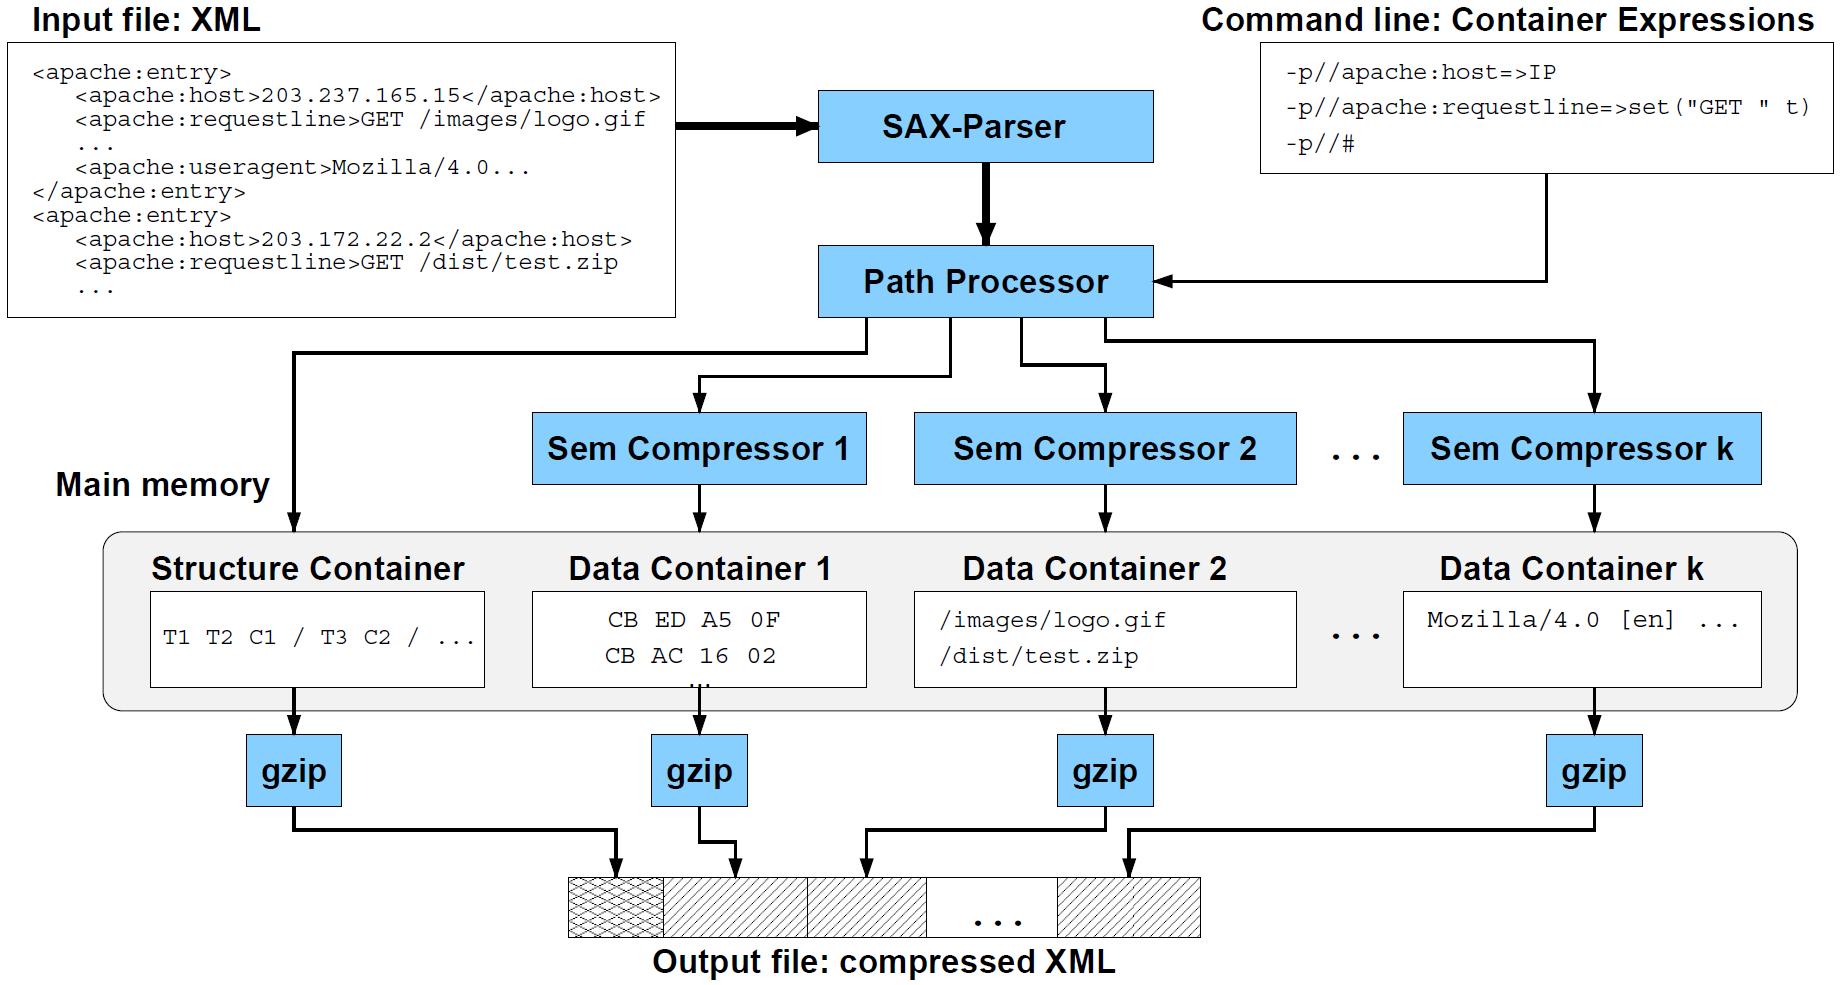
\includegraphics[clip, angle=0, width=150mm]{ArchitekturaXMill}
\caption{Architektura algoritmu XMIll \cite{xmill}}
\label{architekturaXMill}
\end{figure}

\subsection{Oddělení struktury od dat}
\label{xmillOddeleniStruktury}
Struktura XML je složena z tagů a atributů. Počáteční tagy a atributy jsou kódovány slovníkovou metodou a nahrazeny indexem ve slovníku, kladným celým číslem. Ukončující tag je kódován hodnotou 0, při kompresi je díky syntaxi vždy zřejmé, který tak je ukončován. Datové hodnoty jsou nahrazeny záporným indexem kontejneru, do kterého byly přiřazeny.\cite{xmill}

Pro příklad zpracujeme následující informace o článku:

\begin{verbatim}
<article mdate="2011-01-11" key="journals/acta/GoodmanS83">
  <author>
    <name>Nathan Goodman</name>
    <title>Mr.</title>
  </author>
  <title>NP-complete Problems Simplified on Tree Schemas.</title>
</article>
\end{verbatim}

Tagy zde jsou \texttt{article}, \texttt{author} a \texttt{title} a atributy \texttt{mdate} a \texttt{key}. Po zpracování dostaneme výstup \texttt{1 2 -3 3 -4 0 4 5 -5 0 6 -6 0 0 7 -7 0 0}. Lze si povšimnout, že indexování kontejnerů začíná až číslem 3, to proto, že index 0 je rezervován pro kontejner struktury, 1 pro kontejner bílých znaků (umožňuje zachování formátovacích mezer) a 2 pro kontejner obsahující procesní instrukce, DTD a jiné.

\subsection{Seskupení dat stejného významu}
Mapování mezi daty a kontejnery provádí Path procesor na základě cesty k datům (path) a na uživatelem definovaném regulárním výrazu container expression. Základní myšlenkou je hodnotám pro každý tag nebo atribut přiřadit vlastní kontejner. Cesta k datům v příkladě z předchozí části \ref{xmillOddeleniStruktury} vypadá například \texttt{/article/@key} pro atribut a \texttt{/article/author/name} pro tag. Pomocí container expression je možné nastavit pravidla, kdy budou například hodnoty různých tagů ukládány do stejného kontejneru.\cite{xmill}

\subsection{Sémantická komprese}
Jak již bylo zmíněno v úvodu popisu tohoto algoritmu, jsou podporovány 3 druhy sémantických kompresorů: atomické, kombinované a definované uživatelem. Atomických kompresorů je 8, například textový kompresor \texttt{t}, který řetězec pouze zkopíruje na výstup (ten bude později zkomprimován pomocí gzip), nebo kompresor \texttt{u}, který komprimuje kladná celá čísla.

Kombinovaný kompresor je vhodný pro hodnoty, ve kterých lze nalézt nějaký vzor nebo strukturu. Jako příklad lze uvést sekvenční kompresor pro kompresi IP adresy \texttt{seq(u8 "." u8 "." u8 "." u8)}, což znamená sekvenci čtyř kladných celých čísel menších než 256 oddělených tečkou.

Vlastní kompresory lze s výhodou použít na data, která mají strukturu složitou nebo velmi těžce vyjádřitelnou pomocí kombinovaných kompresorů. Autoři jako příklad takových dat uvádějí DNA sekvence. Aby bylo možné data komprimovaná za pomocí vlastní kompresorů zpětně rekonstruovat, musí mít dekompresní algoritmus samozřejmě také přístup k použitému vlastnímu kompresoru.\cite{xmill}